\subsubsection{UART Klassen}

Grænsefladen mellem DevKit8000 og PSoC Masteren blev valgt som UART, grundet tidligere erfaringer med denne type af kommunikation. Der blev designet en UART-protokol (nærmere beskrevet i afsnit \ref{P-sec:UART_protokol} \nameref{P-sec:UART_protokol} på side \pageref{P-sec:UART_protokol} i dokumentationen), som beskriver kommandoer der er nødvendige for systemet. UART klassen virker således som en driver, der håndterer kommunikationen med DevKit8000.

\begin{figure}[h]
\centering 
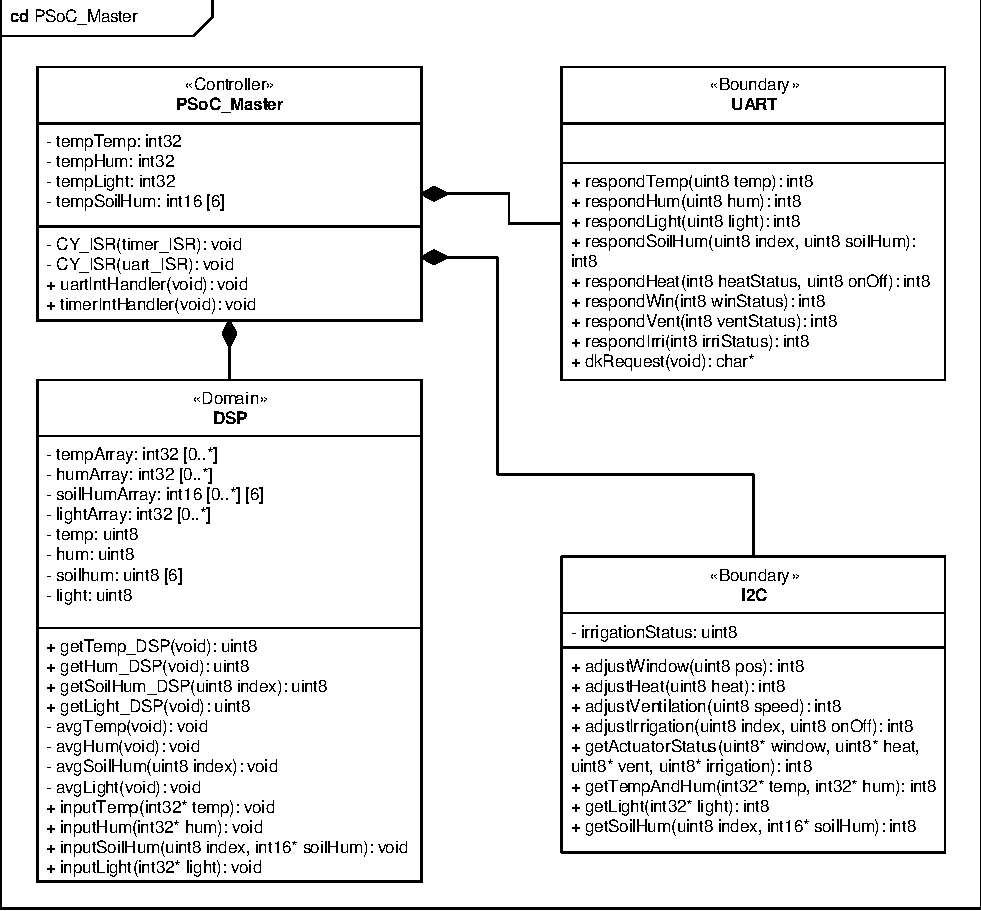
\includegraphics[width=\textwidth * 2/5, trim=269 253 17 30, clip=true] {../fig/cd_PSoC_master.pdf}
\caption{UART klassen}
\label{fig:UART_klasse}
\end{figure}

På Figur \ref{fig:UART_klasse} ses klassediagrammet for UART. Der er designet en public metode, \texttt{dkRequest()}, der sørger for at læse den data, der måtte stå i UART bufferen. Tanken er, at denne metode kaldes fra PSoC Master klassen, når der registres et interrupt. Alle \texttt{respond}-metoderne kaldes med en parameter, der valideres af metoden og hvis denne er gyldig (ikke nul), sendes en passende besked til DevKit8000 jf. UART-protokollen. Eksempelvis sendes \texttt{'X'+'T'}, hvis der er en ugyldig temperatur i DSP-klassens' \texttt{temp} variabel og \texttt{'T'+80} hvis der er målt $20^{\circ}$C med temperatursensoren.